\documentclass[12pt]{article}

\usepackage{tabularx}
\usepackage[a4paper,margin=2.5cm, bottom=3.5cm]{geometry}
\usepackage{fancyhdr}
\usepackage{listings}
\usepackage{booktabs}
\usepackage{float}
\usepackage{subcaption}
\usepackage{graphicx}
\usepackage{amsmath}
\usepackage{amssymb}
\usepackage{amsthm}
\usepackage{array}
\usepackage[table]{xcolor}
\usepackage{pgfplots}
\usepackage{pgfplotstable}
\usepackage{multirow}
\usepackage{tikz}
\usepackage[hidelinks]{hyperref}
\usepackage{titling}
\pgfplotsset{compat=1.17}

\theoremstyle{definition}
\newtheorem*{example}{Example}
\setlength{\headheight}{40pt}
\setlength{\parindent}{0pt}
\setlength{\parskip}{1ex}
\renewcommand{\headrulewidth}{0pt}

\newcommand{\subfiguresize}{.3\textwidth}
\DeclareMathOperator*{\median}{median}

\DeclareMathOperator*{\biggerforall}{\mbox{\Large $\mathsurround0pt\forall$}} 
\DeclareMathOperator*{\bigforall}{\mbox{\large $\mathsurround0pt\forall$}} 
\DeclareMathOperator*{\biggerexists}{\mbox{\Large $\mathsurround0pt\exists$}} 
\DeclareMathOperator*{\bigexists}{\mbox{\large $\mathsurround0pt\exists$}} 

\lstset {
    captionpos = b,
    basicstyle = \small\ttfamily,
    keywordstyle = \color{blue},
    commentstyle = \color{black!30},
    comment = [l]{//},
    morecomment = [s]{/*}{*/},
    identifierstyle=,
    keywords = {
        let,
        mut,
        for,
        in,
        if,
        else,
        continue,
        break,
        pub,
        struct,
        impl,
        type,
        self,
        Self,
        as,
        u8,u16,u32,u64,
        i8,i16,i32,i64,
        f32,f64,
        usize,
    }
}

\pagestyle{fancy}
\fancyhead{}
\fancyhead[L]{
    \renewcommand{\arraystretch}{1.5}
    \begin{tabularx}{\textwidth}{|X|X|}
        \hline
        \large \bf Image processing & \normalsize \thetitle \\
        \hline
    \end{tabularx}
}
\fancyfoot[C]{\thepage}

\renewcommand{\maketitle}{
    \thispagestyle{plain}
    \renewcommand{\arraystretch}{2}
    \vspace*{-7em}
    \begin{flushleft}
        \begin{tabularx}{0.95\textwidth}{|X|X|}
            \hline
            \bf \large Image Processing                   & \bf \large \thetitle                           \\ \hline
            \multicolumn{2}{|l|}{
                \textbf{Task variant:} Group 1
            }                                                                                               \\ \hline
            \textbf{Day and time:} Mon, 14:00             & \textbf{Full name:} \textsc{Jakub Pawlak}       \\
            \textbf{Academic year:} {2022/23} & \textbf{Full name:} \textsc{Magdalena Paku\l a} \\
            \hline
        \end{tabularx}
    \end{flushleft}
    \vspace{1em}
    \renewcommand{\arraystretch}{1}
}
\graphicspath{{../img_task2/}}


\title{Task No.~2}

\begin{document}
\maketitle

\section{Description of the implementation of \texorpdfstring{\\ }{} histogram-based image enhancement method}
Histogram based image enhancements work by assigning new values to the luminosity levels, to match the histogram to some function.
The old luminosities will be denoted as $f$, and the new ones, as $g$.
The histogram of the image is denoted as $H$, and $H(f)$ means the number of pixels with luminosity $f$.
Finally, $N$ will mean the total number of pixels in the image.

\subsection{Mathematical description}

The equation for calculating the new luminosity values were given as:
\begin{equation}
    g(f) = g_{min} +\sqrt{
        2 \alpha^2 \cdot \ln\left[
            \left(
            \frac{1}{N} \sum\limits_{k=0}^f H(k)
            \right)^{-1}
            \right]
    }
    \label{eq:rayleigh-initial}
\end{equation}

We immediately noticed, that the number under the logarithm is a partial sum of the normalized histogram values for luminosities smaller or equal $f$.
We can refactor the equation, by introducing a partial sum function $ps(f)$:
\begin{equation}
    ps(f) = \sum\limits_{k=0}^f H(f)
\end{equation}

Equation (\ref{eq:rayleigh-initial}) then takes form:
\begin{equation}
    g(f) = g_{min} + \sqrt{
        2 \alpha^2 \cdot \ln
        \left(
        \frac{N}{ps(f)}
        \right)}
\end{equation}

Note that,
\(
\bigforall_{f \in \langle f_{min},f_{max}\rangle} : 0 < ps(f) \leq N
\), and $ps(f)$ is monotonically non-decreasing.
That means that $\frac{N}{ps(f)}$ is monotonically non-increasing, and as follows, $g(f)$ is also non-increasing.

However, this is not what we want from image transformation, as it would produce a negative image.
Therefore, we flip the function horizontally, by changing the sign of $ps(f)$, and offsetting it by $N$, to keep the domain the same.

\begin{equation}
    g(f) = g_{min} + \sqrt{
        2 \alpha^2 \cdot \ln
        \left(
        \frac{N}{N - ps(f) + 1}
        \right)}
    \label{eq:rayleigh-corrected}
\end{equation}
Now, as $f$ increases, $g(f)$ will increase as well.

However, the value of $\alpha$ is still unknown.
We know, that the function $g(f)$ should map $f$ to $g$ in such a way, that
$f_{min} \mapsto g_{min}$ and $f_{max} \mapsto g_{max}$.

For the first case:
\(
\lim\limits_{f \to f_{min}} ps(f) = 1
\),which means that
\(
\lim\limits_{f \to f_{min}} g(f) = g_{min}
\) regardless of $\alpha$.

The second case is more interesting:
\begin{align*}
    ps(f_{max}) & = N                \\[1ex]
    g(f_{max})  & = g_{min} + \sqrt{
        2 \alpha^2 \cdot \ln(N)
    }
\end{align*}
Substituting $g(f_{max}) = g_{max}$,
\begin{align}
    g_{max} & = g_{min} + \sqrt{
        2 \alpha^2 \cdot \ln(N)
    }\nonumber                                                                     \\[1ex]
    g_{max} & = g_{min} + \alpha \cdot \sqrt{2\ln(N)} \nonumber                    \\[1ex]
    \alpha  & = \frac{g_{max} - g_{min}}{\sqrt{2\ln(N)}} \label{eq:rayleigh-alpha}
\end{align}

\subsection{Implementation}

We start, by calculating the partial sums of the histogram for each channel:
\begin{lstlisting}
let partial_sums: [[u32; 256]; 3] = {
        let histogram = Histogram::new(image);
        histogram
            .into_iter()
            .map(|h| {
                h.iter()
                    .scan(0u32, |sum, value| {
                        *sum += value;
                        Some(*sum)
                    })
                    .collect()
            })
            .collect::<Vec<[u32; 256]>>()
            .try_into()
            .unwrap()
    };
\end{lstlisting}

\pagebreak[2]
Then, we calculate the image size, and the value of $\alpha$, according to eq. (\ref{eq:rayleigh-alpha})
\begin{lstlisting}
let image_size = image.width() * image.height();
let alpha = (self.gmax - self.gmin) as f64 
    / f64::sqrt(2.0 * f64::ln(image_size as f64));
\end{lstlisting}

\pagebreak[2]
Then, we create the brighness lookup table, according to eq. (\ref{eq:rayleigh-corrected}):
\begin{lstlisting}[basicstyle = \footnotesize\ttfamily]
let mut brightness_lookup = [[0u8; 256]; 3];
for channel in 0..3 {
    for i in 0..256 {
        let partial_sum = partial_sums[channel][i];
        if partial_sum == 0 {
            continue;
        }
        let log_base = 
            image_size as f64 / (image_size - partial_sum + 1) as f64;
        let root_base = 
            2.0 * alpha * alpha * f64::ln(log_base);
        brightness_lookup[channel][i] = 
            self.gmin
            + f64::clamp(
                f64::sqrt(root_base), 
                0.0, 
                (self.gmax - self.gmin) as f64) as u8;
        if partial_sums[channel][i] == image_size {
            break;
        }
    }
}
\end{lstlisting}

Note 2 important things --- the \lstinline{continue} and \lstinline{break} statements inside the loop.
We are interested in filling the lookup table only for values of $f \in \langle f_{min}, f_{max} \rangle$.
Therefore, we check if $ps(f) = 0$. If it is, then $f < f_{min}$, and we need not perform the calculation, so we continue looping
until we encounter some $ps(f) > 0$.

Similarly, we do not need to perform calculations for $f > f_{max}$. We know that $ps(f) = N \Leftrightarrow f \geq f_{max}$,
so if we reach that point, we do not need to perform any calculations for further values of $f$, and can safely break out of the loop.

This is a small optimization compensating for the fact that we cannot create a smaller lookup table, adjusted to the size of $\langle f_{min}, f_{max}\rangle$, because these values are unknown at compile time.

\pagebreak[2]
Finally, we set the new luminosity levels in the image according to the created lookup table:
\begin{lstlisting}
for pixel in image.pixels_mut() {
    for channel in 0..3 {
        let luminosity = pixel[channel];
        let new_luminosity = 
            brightness_lookup[channel][luminosity as usize];
        pixel[channel] = new_luminosity
    }
}
\end{lstlisting}


\section{Image analysis on the basis of the histogram}
\subsection{Implementation}

After conducting an image improvement by using Rayleigh distribution described in the previous section, we could see tremendous differences presented below.

In order to obtain that result, we chose those input numbers as an example.
\begin{align*}
    g_{max} & = 1                                                                     \\[1ex]
    g_{max} & = 200                    
\end{align*}

\subsection{Results}
\begin{figure}[H]\centering
    \begin{subfigure}[t]{\subfiguresize}\centering
        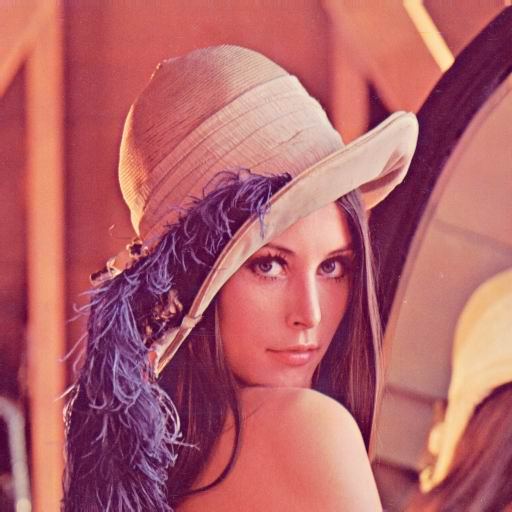
\includegraphics[width=\textwidth]{lenac.png}
        \caption{original}
    \end{subfigure}
    \hspace{.05\textwidth}
    \begin{subfigure}[t]{\subfiguresize}\centering
        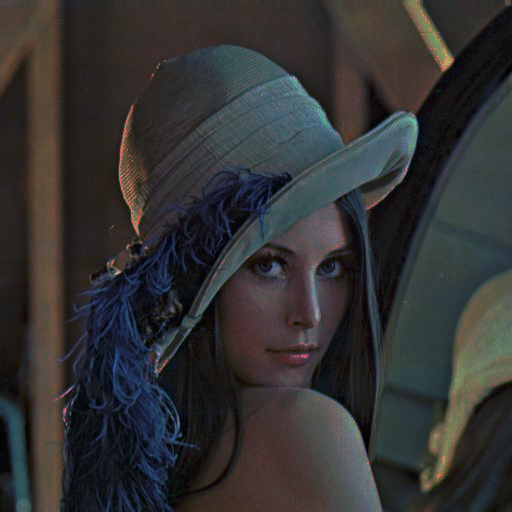
\includegraphics[width=\textwidth]{lena_hraleigh_1_200.png}
        \caption{modified}
    \end{subfigure}
    \caption{Image before and after Rayleigh distribution}
\end{figure}

\begin{figure}[H]\centering
    \begin{subfigure}[t]{\subfiguresize}\centering
        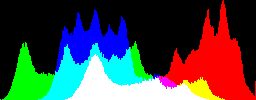
\includegraphics[width=\textwidth]{lena_clear_histogram.png}
        \caption{original}
    \end{subfigure}
    \hspace{.05\textwidth}
    \begin{subfigure}[t]{\subfiguresize}\centering
        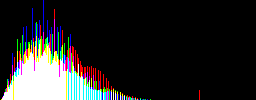
\includegraphics[width=\textwidth]{lena_hraleigh_1_200_histogram.png}
        \caption{modified}
    \end{subfigure}
    \caption{Histogram before and after Rayleigh distribution}
\end{figure}
\subsection{Complex analysis}

As we can see, the difference is huge. the output picture is less red and more neutral for the viewer. The same difference we can observe on the histogram created on the before and after picture. While on the original image most of the colors are taking the whole histogram and only part of them are interfering with each other, on the modified picture almost all the colors are interfering, which resulted in very neutral picture for the viewer, which is not that diverse in colors. The histogram of the original image has majority of the red channel, which can be seen on the original image as having red undertones. On the histogram of the modified picture came out with majority of blue tones, which can be clearly seen on the image. These comparisons can perfectly present a fully working histogram on all the channels at the same time.

\subsection{Characteristics analysis}

In this project we implemented and tested all 8 different characteristics for image transformations which are:
\begin{itemize}
  \item Mean and Variance
  \[ b=\frac{mH_A(m)}{N\sum_{L-1}^{m=0}}\]
   \[ D^2=\frac{(m-b)^2H_A(m)}{N\sum_{L-1}^{m=0}}\]
  \item Standard deviation and Variation coefficient I 
   \[ \sigma _x=\sqrt{}D^{2}\]
    \[ b_z= \frac{\sigma _x}{b}\]
  \item Asymmetry coefficient
   \[ b_s=\frac{(\frac{1}{\sigma ^3})(m-b)^3H_A(m)}{N\sum_{L-1}^{m=0}} = \frac{(m-b)^3H_A(m)}{\sigma ^3N\sum_{L-1}^{m=0}}\]
  \item Flattening coefficient
   \[ b_K=\frac{(\frac{1}{\sigma ^4})(m-b)^4H_A(m)-3}{N\sum_{L-1}^{m=0}} = \frac{(m-b)^4H_A(m)-3}{\sigma ^4N\sum_{L-1}^{m=0}}
\]
  \item Variation coefficient II
   \[ b_N=\frac{[H_A(m)]^2}{(N\sum_{L-1}^{m=0})^2}\]
  \item Information source entropy
   \[ b_I=-1\frac{H_A(m)log_2(\frac{H_A(m)}{N})}{N\sum_{L-1}^{m=0}}\]
\end{itemize}

For all of the calculations we used formulas available on the Task 2 exercise on Wikamp. The result of all of those calculations for the original and modified picture are presented below in the table.

\section{Description of the linear filter implementation}

\subsection{General formulation}

\subsubsection{Mathematical description}

The linear filter implementation is based on the principle of convolution of the mask $3\times3$ matrix $\mathbf{M}$, with an image fragment of the same size.

Consider a following mask:
\begin{equation}
    \mathbf{M} = \begin{bmatrix}
        a_{0,0} & a_{1,0} & a_{2,0} \\
        a_{0,1} & a_{1,1} & a_{2,1} \\
        a_{0,2} & a_{1,2} & a_{2,2}
    \end{bmatrix}
\end{equation}

Then, for each pixel at coordinates $(x,y)$, we will compute its new value as
\begin{equation}
    g(x,y) = \sum\limits_{i=0}^2 \sum\limits_{j=0}^2 a_{i,j} \cdot f(x + i - 1, y + j - 1)
\end{equation}

Note, that we have to subtract 1, so the pixel $f(x,y)$ will correspond to the center of the $\mathbf{M}$ matrix ($a_{1,1}$).

Important thing, is that for pixels on the edges,
the convolution with $\mathbf{M}$ would require calculating values of pixels outside of the image, which is impossible.
Therefore, for such cases, we assume $g(x,y) = f(x,y)$.

\subsubsection{Implementation}

During the implementation, we noticed that it is sometimes more convenient
to have a separate factor to multiply the matrix with.
For example:
\[
    \mathbf{M} = \begin{pmatrix}
        4 & 2 \\ 2 & 4
    \end{pmatrix} = 2 \begin{pmatrix}
        2 & 1 \\ 1 & 2
    \end{pmatrix}
\]

Moreover, we can factor this value out of the sum, to reduce the number of necessary operations.
Therefore, in our filter settings we store 2 fields: the mask matrix, and the mask scale factor.
When running the program, the user is asked to provide the mask as a command line argument.
They can also provide the optional mask scale (which by default will be set to 1).
This way, it is much more convenient for the user to input masks that have fractional values (like the low-pass filter masks).

Finally, like with all transformations that operate on more than one pixel at a time,
it is necessary to allocate a new image buffer, as to not corrupt the data in the original one.

Having done all this preparation, we are ready to implement the convolution, while remembering to skip the edge pixels:

\pagebreak[3]
\begin{lstlisting}
for (x, y, pixel) in new_image.enumerate_pixels_mut() {
    if is_edge(image, x, y) {
        *pixel = *image.get_pixel(x,y);
        continue;
    }
    for channel in 0..3 {
        let mut sum: f64 = 0.0;
        for i in 0..3 {
            for j in 0..3 {
                sum += (self.mask[j][i])
                    * image.get_pixel(x+i-1, y+j-1)[channel];
            }
        }
        pixel[channel] = (sum * self.mask_scale) as u8;
    }
}
\end{lstlisting}

\paragraph{Important remark}
At the time of writing this report, it was noticed, that although we were supposeed to implement just the low-pass filter,
since the user has the ability to provide any $3\times3$ mask in the command line,
there is nothing stopping them from inputing the mask for e.g.\ line identification or edge sharpening.
Therefore, our implementation actually works not for just low-pass filter, but for all the convolution-based filters with a $3\times3$ mask.

\subsection{With optimization}

\subsubsection{Reasoning}

Looking at the unoptimized implementation of the filter, it was difficult to find the ways of further optimization.
The extraction of the scale factor, already reduced the number of multiplications.
We could optimize the first low-pass filter mask, as it has all 1's in the mask, which would further reduce the number of multiplications,
However, we do not think that it would give such a great performance boost.
We could also, utilize the fact, that the mastrix size is constant, and eliminate the for loops, adding the values manually, since there are only 9 of them.
This would eliminate unnecessary bounds checks on the loop indexes.
However, since the loop ranges are a compile-time constans, the compiler would already perform this optimization (we checked both options and looked at the decompiled code).
Moreover, this could prevent the compiler from doing optimizations specific for loops, such as loop vectorization.

Therefore, we decided to take a completely different approach, and instead of changing the code, we changed the processing unit.
Instead of doing the computations on the \textsc{cpu}, which does the operations sequentially (except some optimizations utilizing the \textsc{simd} instructions),
we moved the computation to the \textsc{gpu}, which is much better at performing simple calculations in parallel.
Since we create the new image buffer, the original image would be read only, and each compute kernel would write to only one pixel of the output image,
this soulution will have no race conditions and be safe to implement as a parallel computation.

\subsubsection{Implementation}
The optimized version would be implemented similarly to the \textsc{gpu}-accelerated filters from the previous task.
We would use Vulkan API to run a compute shader containing the convolution code.

We set the working group size to $16\times16$ pixels, as it is a standard size for processing images,
and we found it to work quite well during previous implementations.
We will provide the shader with the mask as a push constant, so \emph{the optimized version will also work for any $3\times3$ mask}.

\begin{lstlisting}[
    basicstyle=\footnotesize\ttfamily,
    morekeywords={
        float,
        layout,
        in,
        uniform,
        readonly,
        writeonly,
        image2D
    }
]
layout (local_size_x=16, local_size_y=16, local_size_z=1) in;

layout (push_constant) uniform PushConstantData {
        float[9] mask;
} dat;

layout (set=0, binding=0, rgba8) uniform readonly image2D inImg;
layout (set=0, binding=1, rgba8) uniform writeonly image2D outImg;
\end{lstlisting}

The shader will convert the mask to \lstinline{mat3}, which is a builtin type representing a $3\times3$ matrix.
Then, it will collect the luminosity values of the neighboring pixels, also to \lstinline{mat3}.

Finally, it will compute the hadamard product of the 2 matrices using a built-in function \lstinline{matrixCompMult()} (\href{https://registry.khronos.org/OpenGL-Refpages/gl4/html/matrixCompMult.xhtml}{see documentation}).
The final result is the sum of all the elements of the resulting matrix.

\begin{lstlisting}[
    language=C++,
    morekeywords={
        vec3,
        ivec2,
        mat3
    }
]
vec3 convolution(mat3 mask, ivec2 xy)
{
    vec3 pixel;

    // Extract a 3x3 region centered in xy
    mat3[3] region = region3x3(xy);

    // for each color channel of region
    for (int i = 0; i < 3; i++)
    {
        mat3 rc = region[i];
        mat3 c = matrixCompMult(mask, rc);
        // add each component of matrix
        float r =  c[0][0] + c[1][0] + c[2][0]
                 + c[0][1] + c[1][1] + c[2][1]
                 + c[0][2] + c[1][2] + c[2][2];

        pixel[i] = r;
    }

    return pixel;
}
\end{lstlisting}

\subsection{Time comparison}

For greater reliability, we run the tests on the bigger image size ($2560 \times 2560$).
Each implementation was run 3 times, and the average execution time was calculated. The results are shown in table \ref{tab:lowpass-execution-time}.

\begin{table}[h]\centering
    \begin{tabular}{ccc}
        \toprule
        Test N\textsuperscript{\underline{o}} & unoptimized & optimized \\\midrule
        1                                     & 12.983      & 3.555     \\
        2                                     & 12.996      & 3.465     \\
        3                                     & 12.975      & 3.453     \\\midrule
        \bf avg.                              & 12.985      & 3.491     \\
        \bottomrule
    \end{tabular}
    \caption{Results of testing the execution times of unoptimized and optimized versions of low-pass filter.
        The time values are given in seconds.}
    \label{tab:lowpass-execution-time}
\end{table}

As we can see, there is a clear difference in the execution times. 
The standard version took almost 13s to execute, while its optimized counterpart performed in less than 3.5 seconds.
This is a huge increase in the execution speed; the optimized version is over 370\% faster than the standard one.

\section{Analysis of the filtering results (linear filter)}

\section{Description of the non-linear filter implementation }

\section{Analysis of the filtering results (non-linear filter)}
\subsection{Results}
For our project we were given Uolis operator filtration. In order to analyse the results we conducted this process on three different images: without a noise, with normal noise and with uniform noise. The results are presented below.

\begin{figure}[H]\centering
    \begin{subfigure}[t]{\subfiguresize}\centering
        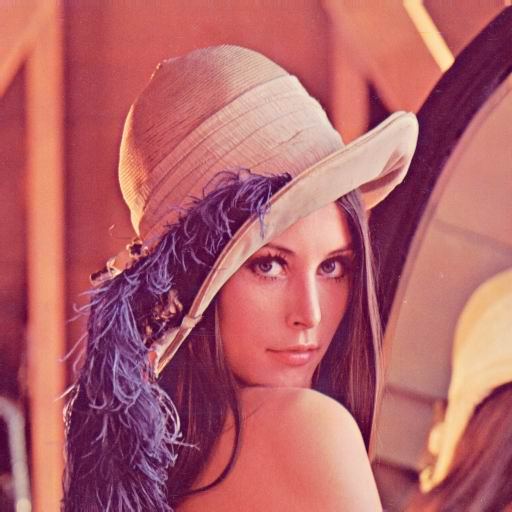
\includegraphics[width=\textwidth]{lenac.png}
        \caption{original}
    \end{subfigure}
    \hspace{.05\textwidth}
    \begin{subfigure}[t]{\subfiguresize}\centering
        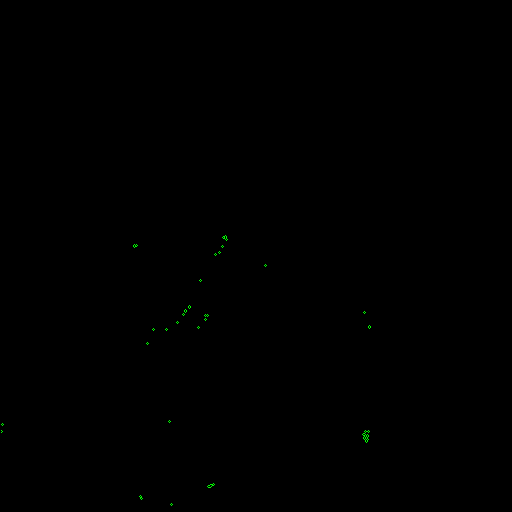
\includegraphics[width=\textwidth]{lena_uolis_clear.png}
        \caption{modified}
    \end{subfigure}
    \caption{Image without noise before and after Uolis operation}
\end{figure}

\begin{figure}[H]\centering
    \begin{subfigure}[t]{\subfiguresize}\centering
        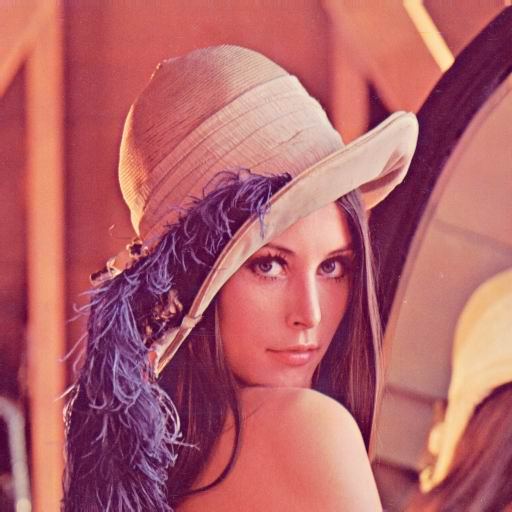
\includegraphics[width=\textwidth]{lenac.png}
        \caption{original}
    \end{subfigure}
    \hspace{.05\textwidth}
    \begin{subfigure}[t]{\subfiguresize}\centering
        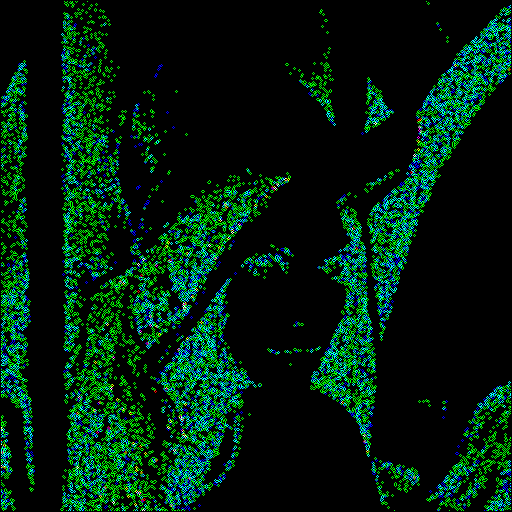
\includegraphics[width=\textwidth]{lena_uolis_normal.png}
        \caption{modified}
    \end{subfigure}
    \caption{Image with normal noise before and after Uolis operation}
\end{figure}

\begin{figure}[H]\centering
    \begin{subfigure}[t]{\subfiguresize}\centering
        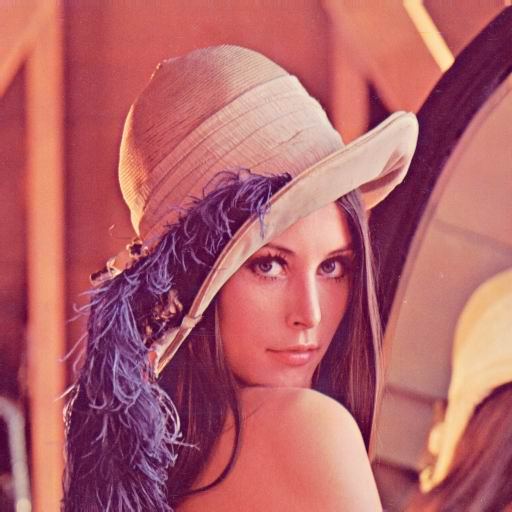
\includegraphics[width=\textwidth]{lenac.png}
        \caption{original}
    \end{subfigure}
    \hspace{.05\textwidth}
    \begin{subfigure}[t]{\subfiguresize}\centering
        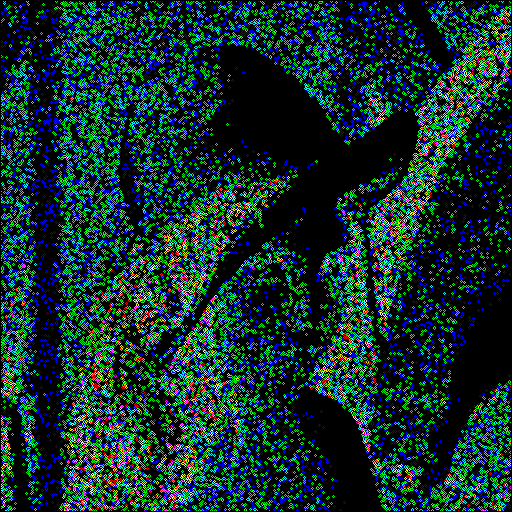
\includegraphics[width=\textwidth]{lena_uolis_uniform.png}
        \caption{modified}
    \end{subfigure}
    \caption{Image with uniform noise before and after Uolis operation}
\end{figure}

\subsection{Complex analysis}

As we can see the results differed between each other because of input images and their lack or not of noise. The biggest noticeable difference we can spot on the image with uniform noise. 

\section{Description of other changes which took place in the application}

During our project we divided the work equally, which enabled us to work faster and more efficiently. When it comes to the application itself we created unit tests for our calculations in order to avoid mistakes. Those tests quickly came to use, because of minor difficulties with mathematical equations. We also tried to do as much as we can operations on GPU instead of only CPU, which resulted in differences in running time and broadened our knowledge in coding.


\vfill
\section*{Teacher's remarks}
\begin{tabularx}{\textwidth}{|X|}
    \hline
    \vspace{7cm}
    \phantom{.} \\
    \hline
\end{tabularx}

\end{document}